
\hypertarget{abduction-resiliency-and-the-weight-of-evidence-1}{%
\chapter{Abduction, Strategic Interrogation, and The Weight of
Evidence}\label{ch:woe}}



The main purpose of this chapter is to propose a way in which the interplay between abduction and deduction can be understood, in service of understanding how the deliberative elements of an experiment could be criticized. The process of abduction, I suggest, is intertwined with deduction: deduction is used to strategically interrogate the hypothesis chosen provisionally, in order to see a better hypothesis should be chosen before committing into inductively testing the hypothesis. During deliberation, we switch back and forth between making educated guesses abductively and derive the necessary connections from it deductively. 

To see how this is done in the context of probabilistic judgment, I shall examine Keynes' notion \emph{the weight of evidence}. My claim is that the weight of evidence is a \emph{deductive} tool a reasoner could use to evaluate the worthiness of a provisionally chosen hypothesis. In particular, I suggest that the intentions and goals of an experimenter can be criticized by appealing to notions of \emph{counterfactual priors and hypothetical data}. My suggestions here are heavily influenced by the works of statisticians
who have argued to move away from the orthodox approaches to Bayesian
analysis, such as James Berger's ``Robust Bayesianism'',\footnote{\cite{robust}} Gelman and
Shalizi's ``hypothetico-deductive Bayesianism'',\footnote{\cite{gelman}} and Peter Walley's theory of imprecise probability.\footnote{\cite{walley}}



I will set the stage with a discussion on Peirce's idea that abduction is an interrogative process in section \ref{strategicint}. An exposition on Keynes' ideas on the weight of evidence will be carried out in section \ref{the-weight-of-evidence-1}. To motivate my proposal, I will introduce Popper's \emph{paradox of ideal evidence} in \ref{the-paradox-of-ideal-evidence-1}. I will overview a statistical solution to the paradox in section \ref{the-statistical-perspective-1}, and a formal epistemological perspective in \ref{the-concept-of-resiliency-1}. Finally, I will articulate my proposal in \ref{counterfactual-priors-and-hypothetical-data-1}.

\section{Deduction as Strategic Interrogation}\label{strategicint}

In section \ref{sec:the-abductive-context-of-inquiry}, we discussed Peirce's idea that the abduced hypothesis is a highly fallible conjecture, insofar so he would sometimes refer to it as a guess. However, Peirce also makes it clear that, even though abduction is ultimately guessing, he does not mean that abduction is nothing but a game of blind luck. One characterization that Peirce often use in the context of abduction is that it involves an ``interrogation'':

\begin{quote}
	A hypothesis ought, at first, to be entertained interrogatively. \footnote{\cite{CP}, 6.524}
	
	The first starting of a hypothesis and the entertaining of it, whether as a simple interrogation or with any degree of confidence, is an inferential step which I propose to call abduction.	 \footnote{\cite{CP}, 6.525}
	
	It is to be remarked that, in pure abduction, it can never be justifiable to accept the hypothesis otherwise than as an interrogation. But as long as that condition is observed, no positive falsity is to be feared; and therefore the whole question of what one out of a number of possible hypotheses ought to be entertained becomes purely a question of economy.	\footnote{\cite{CP}, 6.529}
\end{quote}

A helpful way to explain what Peirce means by ``interrogation'' is to use own analogy of the game of ``twenty questions'', in which one party has to think of an object, while another party has to find out what the object by asking 20 or less questions.\footnote{\cite{essentialpeirce2}, 109} Peirce's idea is that posing a question in the game is akin to proposing a hypothesis in an inquiry---for both cases, we make a guess about the nature of the subject of our inquiry, and the difference is that in the game the answer we receive is certain and direct, while a hypothesis has to be tested or broken down into sub-hypothesis. Peirce has an important point in mind, however, with this example. That is, the choice of the question to ask can drastically alter the course of an inquiry. Since the player of the game has to figure out what the answer is by asking at most 20 questions, she must ask them \emph{strategically}. Each question the inquire asks should be as informative as possible---they should, for instance, ask questions that narrow the space of possibilities as quickly as possible. Abduction, which is the logic of hypothesis selection, is guided by a similar goal.

Hintikka, who calls abduction ``the fundamental problem in contemporary epistemology'', proposes that the interrogative element of abduction could be understood as the strategic process in which the informational gain, in light of the agent's epistemic goal, from inquiry is maximized.\footnote{\cite{hintikka}} Hintikka raises an interesting example of how the strategic freedom in abductive thinking is crucial for deductive logic, notwithstanding its emphasis on mechanical rules of inference. Suppose a student is asked, in an exam for a logic class, to demonstrate that

\begin{equation}
	\vdash [[A\to(B\wedge \neg C)] \wedge (\neg B \vee D) ]\to (A\to D)
	\label{eq:abdeexample}
\end{equation}

 
 
 In other words, the student has to prove that formula \ref{eq:abdeexample} is a logical truth. Before proving that, she must make a decision on which method to use. Since she is pressed for time, it is in her interest to prove in a strategic manner. For instance, suppose she choose the \emph{semantic} strategy of showing that the proposition is  always true. The most obvious way would be to use the truth table to show that the formula is true under all possible interpretations. However, that would be a inefficient choice, since there will be $2^4=16$ rows and, because of her strategic decision, she cannot skip any row---she has to demonstrate that the proposition is true in all rows. 


Thus, the strategic dimension of reasoning involves finding a way to gain as much information as possible in light of economical constraints. In the game of twenty questions, the constraint is that the questioner only gets 20 questions. For the student taking the logic exam, her time is obviously limited. In each of the cases, before even tackling the problem that confronts her, the reasoner has to deliberate on how to go about solving the problem, such as choosing from one of many methods in which the problem could be addressed. Reasoning about how our resources should be allocated in service to our epistemological goal is often categorized by Peirce as the logic of the economy of research:

\begin{quote}
Proposals for hypotheses inundate us in an overwhelming flood, while the process of verification to which each one must be subjected before it can count as at all an item, even of likely knowledge, is so very costly in time, energy, and money---and consequently in ideas which might have been had for that time, energy, and money, that Economy would override every other consideration even if there were any other serious considerations. In fact there are no others.\footnote{\cite{CP}, 5.602}	
\end{quote}

Hinttika's point the connection between abduction and deduction is relevant here. The economical implication of a hypothesis can often be probed in a deduction, which is both relatively cost-free and secure. 

For example, reconsider formula \ref{eq:abdeexample}. Let's say the logic student realizes that using truth table would be uneconomical for this particular problem, and decides to use natural deduction instead. This, however, calls more further strategic thinking, because since there is no premise given, the student must \emph{choose} her own assumed premise, and often there are many different ways in which a proof can begins . Introductory textbooks often recommend the strategy of  assuming the negated version of the logical truth, and prove the result by using \emph{Reductio ad Absurdum}, if the student is unsure how to begin.

 In this case, however, this might not be the best decision, for the result seems rather unwieldy:
 
 \begin{equation}
	  \neg \{[[A\to(B\wedge \neg C)] \wedge (\neg B \vee D) ]\to (A\to D)\}\vdash ????
	\label{eq:abdeexampleneged}
\end{equation}

She would end up with a long negated conditional, without a clear way forward. Of course, it is not impossible to find a contradiction from  formula \ref{eq:abdeexampleneged}. If the student keeps out unpacking it deductively, she will eventually run into a contradiction by brute force, just as in the game of twenty questions, a player might eventually run into the correct answer if she had unlimited chances to ask question. 

But there are possibly more economical ways to start the. proof.  One strategy would be to take advantage of the conditional nature of the logical truth. That is, we can prove the result conditionally assuming the antecedent of the conditional, and derive the consequent:

\begin{equation}
	 [[A\to(B\wedge \neg C)] \wedge (\neg B \vee D) ]\vdash (A\to D)
	\label{eq:abdecp}
\end{equation}

The right hand side of the $\vdash$ presents itself a clear way forward: assume $A$, and then derive $D$.  A student with a keen eye for deduction can see that the assumption given in \ref{eq:abdecp} is a conjunction that can be decomposed into two conjuncts, giving us the propositions needed to derive $B\wedge \neg C$ using $A$, and then get $D$, using $B\wedge \neg C$.  Depending on the rules available to her, such a method would take 10 or less lines. Of course, this is not to say there is an \emph{a priori} reason to prefer the conditional strategy over the \emph{reductio} strategy. The rationality of these choices are highly sensitive to the context of the problem, informed by, for instance, the reasoner's ability. 

 Similar considerations apply in the game of twenty questions. Suppose we are considering for the first question the choice between asking "is it steak?" and "is it food?" It is a matter of deduction that the latter is much more informative: both an affirmative or negative answer would greatly reduce the size of the possible question. It would, of course, be nice if the answer happens to be steak, in which case the former would be the question to ask, but the probability, given we know nothing about the object in question, is astronomically low, and knowing that it is \emph{not} steak only rule out \emph{one} possible answer. 

These examples are intended to serve as an intuitive analogy to the main idea I wish to develop in this chapter is the interplay between abductive and deductive reasonings in inquiry: in particular, how non-evidential but epistemologically relevant questions such the economy of a proposed premise can be investigated deductively. Nevertheless, our discussion here brings light to an important idea that has been implicit in the dissertation: during deliberation, abduction and deduction are quite interwoven: there is not a discrete point to which we can point and say that the investigator has moved on from the abductive stage to the inductive stage. After deduction draws out the necessary connections from a provisionally chosen hypothesis, the inquirer must consider that the now explicit implications of her initial choice bear on her goals, intentions, and values. She may decide to revise her initially decision based on this new information, and she may again use deduction to tease out the repercussions of her informed decision. This highlights the interrogative role deduction plays in inquiry. Lastly, this dynamic relationship between abduction an deduction is one of the reasons why I have chosen to put both under the heading of deliberation, because it is often impossible to separate them in practice.      	
%
%The creative and suggestive nature of abductive inference makes it permissive in nature, and, for it to be reliable, it must be guided by economical considerations that discriminate between productive and unproductive proposals. According to the schema Peirce provides, we can infer that there is a reason to suspect a hypothesis to be true, as long as it accounts for the facts somehow. To be sure, Peirce makes it clear that the permissive nature of abduction must be tempered by the pragmatic maxim---a hypothesis must be distinguishable by their experimental and practical consequences.[@essentialpeirce2 234] Still, for many facts, there could be countless possible testable accounts, and examining every single possible abductive suggestion is not only imprudent, but it impedes greatly our ability to find the right hypothesis.[@CP 2.776] Thus, how to deal with this problem, in light of our limited resources, is the heart of the economy of research and the rationality of abduction:
%



\hypertarget{the-weight-of-evidence-1}{
\section{The Weight of Evidence}\label{the-weight-of-evidence-1}
}

In \emph{A Treatise in Probability}, Keynes discusses a great deal about
how probability ought to reflect our epistemic judgments. One type of
such judgments is the \emph{judgment of relevance}. Keynes' observation
is that we often can judge whether one proposition \(E\) counts as being
relevant to another proposition \(H\) by considering whether the
probability of \(H\) would change on the supposition that \(E\) is true.
Keynes's example is that, in a typical urn example with some black and
white balls, if we want to know the probability of a white ball being
randomly chosen, the color of the ball would not change its probability
of being chosen, so the idea is that a ball's probability of being
chosen conditional on being (say) white is the same as the probability
of the ball being chosen in general.\footnote{Keynes, \emph{A Treatise
  on Probability}, 59.} So, Keynes proposes that evidence \(E\) is
irrelevant to the proposition \(H\) if and only if:

\[P(H|E ) \neq P(H) \]

However, Keynes is troubled by the fact that the
degree of a probability does not scale straightforwardly with the amount
of the evidence we have at hand. In a well-known passage, Keynes says:

\begin{quote}
As the relevant evidence at our disposal increases, the magnitude of the
probability of the argument may either decrease or increase, according
as the new knowledge strengthens the unfavourable or the favourable
evidence; but something seems to have increased in either case,---we
have a more substantial basis upon which to rest our conclusion. I
express this by saying that an accession of new evidence increases the
weight of an argument. New evidence will sometimes decrease the
probability of an argument, but it will always increase its `weight.'
\end{quote}

The crucial idea here is the weight of evidence is closely tied to the
absolute amount of evidence and is conceptually distinct from the
``magnitude'' of a probability. Keynes explains this as the distinction
between the \emph{balance} and the \emph{weight} of the evidence: he
first brings our attention to the fact that when we consider the
conditional probability of the hypothesis in question under all relevant
evidence, the resultant number constitutes the balance between favorable
and unfavorable evidence.\footnote{Keynes, 78.} For instance, we may say
that when \(P(H)<0.5 <P(H|E)\), then evidence \(E\) is somewhat in favor
of the hypothesis. Of course, the balance changes as we gather more
relevant evidence, and it might go from favorable from unfavorable
depending on the nature of the new evidence.

However, as Keynes points out, this is not the only epistemologically
significant relation between probability and evidence, for we not only
care about how much the current evidence favors the hypothesis, but we
also concern ourselves with the \emph{amount} of evidence involved in
calculating the balance of the evidence, and Keynes calls this measure
the \emph{weight} of evidence. But, unlike the balance of the evidence,
which can go either direction, the weight of evidence can only go up as
we gather more relevant evidence. In Keynes' words, ``New evidence will
sometimes decrease the probability of an argument, but it will always
increase its `weight.'\,''\footnote{Keynes, 78.}

To see what Keynes means, imagine two urns \(A\) and \(B\) with unknown
proportions of black and white balls. Suppose you sample (with
replacement) 100 balls from the urn \(A\) and find 50 black balls and 50
white balls. Justifiably, you infer that the proportion of black balls
in \(A\) - call it \(\theta_A\) is about \(0.5\). You then decide to
sample from \(B\), but this time you only manage to draw 4 samples, 3 of
which are black balls. Your best estimate for \(\theta_B\) is \(0.75\).
At this point, I offer you another chance to draw from one of the urns,
and if you manage to draw a black ball from that urn, you get \$100.
Which urn would you pick?

Clearly, \(\theta_B > \theta_A\), but it is not clear that \(B\) is
obviously the better choice, because the amount of evidence you have for
\(\theta_A = 0.5\) is higher than for \(\theta_B = 0.75\). This is a
problem for probabilism, because, in terms of just comparing the
probabilities alone, picking urn \(B\) clearly has a higher probability
of winning; however, all the facts in the situation are different than
what the probability lets on, so the probability has failed to reflect
some crucial information about the evidence.

Keynes was not the first to notice the problem of the weight of
evidence, it is one of many criticisms Peirce has for what he calls
\emph{conceptualism}, a subjective position on probability that was
heavily influenced by Laplace. In particular, conceptualists accept of
the so-called Principle of Indifference, which says roughly that
complete ignorance should be modeled as a uniform distribution over all
hypotheses. In a typical case of estimating a unfamiliar coin's
probability of heads, this would mean that the expected value is
\(0.5\).

We already reviewed some of Peirce's problems with the Principle of Indifference in section \ref{rational-degrees-of-belief}. It is in this context that
Peirce appeals to the notion of the weight of evidence. Peirce's argument is pragmatic: conceptualists say that you should
adhere to the Principle of Indifference when you either have no
information. This means that the degree of belief you \emph{should} have
for a unfamiliar coin landing on heads on the next toss is 0.5. However,
Peirce argues there is a behavioral difference between betting on a fair
coin and a unfamiliar coin. For the former you should know exactly how
much to bet, in the latter case you should simply refrain from betting.
The Conceptualist model, however, cannot make sense of this, since both
entail the degree of belief of \(0.5\). Nowadays this is usually known
as the \emph{Ellsberg's Paradox}.\footnote{Ellsberg, ``Risk, Ambiguity,
  and the Savage Axioms.''}

In other words, conceptualism fails to distinguish between
\emph{rational indecision} and \emph{indifference}. What distinguishes
the two is the difference in the weight of evidence. To recycle the
example earlier, further consider another urn \(C\), from which you draw
2 balls, and one of them is white, so your best estimate would be
\(\theta_c = 0.5\). If probabilities can perfectly reflect the evidence,
then it must mean that your epistemic attitude toward \(A\) and \(B\)
ought to be the same, but Peirce insists that this cannot be the case.

\begin{quote}
In short, to express the proper state of our belief, not one number but
two are requisite, the first depending on the inferred probability, the
second on the amount of knowledge on which that probability is based.
\end{quote}

The weight of evidence, then, is a crucial piece of the puzzle for the
position I am trying to defend. The goal of Deliberative Bayesianism
aims to situate Bayesianism within the Peirce's framework of abduction,
deduction, and induction. My claim is that the weight of the evidence something is relevant in \emph{abduction}. This is why Keynes was perplexed about it. 

\hypertarget{the-paradox-of-ideal-evidence-1}{%
\section{The Paradox of Ideal
Evidence}\label{the-paradox-of-ideal-evidence-1}}

Like Peirce before him, Karl Popper was highly critical of the
subjective interpretation of probability and the epistemologies that
sprung out of it. Popper has further develop Peirce's criticism as the
\emph{paradox of ideal evidence}. The alleged paradox arises out of the
contradiction that, by accepting the notion of conditional relevance
proposed by Keynes, some evidence is both relevant and irrelevant.

Popper asks us to consider a certain coin with an unknown bias: let
\(N\) be the proposition ``the next toss of the penny will yield
heads.''\footnote{\cite{popperlogic}, 425.}
Now, what should \(P(N)\) be? He suggests, either by appealing to
intuition or the Principle of Indifference, Bayesians would suggest that
\(P(N) = 0.5\).\footnote{It should be noted that Popper is not attacking
  the principle of indifference in this context. That is, for this
  argument he is willing to grant that Bayesians have some way of
  arriving at \(P(N)\)---it could be by indifference, through
  elicitation, etc.}

Now let \(I\) be what he calls \emph{the ideal statistical evidence} in
favor of the idea that the coin in question is a fair one. Popper's
example is to let \(I\) be a statistical report that says `in a million
tosses, the coin landed on heads roughly half a million times.' The
exact number is not important, as long as the number of heads and tails
would make it practically certain that the coin is fair---the same point
could be made using 10 millions instead of a million. Now, given we have
ideal evidence \(I\), what is the probability of \(N\)? Popper claims
that it would have to be \(1/2\). So

\[P (N|I) = P(N) = \frac{1}{2}\]

\noindent However, as discussed earlier, evidence \(I\) is relevant to
the hypothesis \(N\) if and only if

\[ P(N|I) \neq P(N) \]

\noindent If \(P(N|I) = P(N) = 1/2\), this means that the ideal evidence
is also irrelevant evidence. Popper then concludes:

\begin{quote}
Now this is a little startling; for it means, more explicitly, that our
so-called `degree of rational belief' in the hypothesis, {[}\(N\){]},
ought to be completely unaffected by the accumulated evidential
knowledge, {[}\(I\){]}; that the absence of any statistical evidence
concerning {[}the hypothesis that the coin is fair{]} justifies
precisely the same `degree of rational belief' as the weighty evidence
of millions of observations which, prima facie, support or confirm or
strengthen our belief.\footnote{Popper, 426.}
\end{quote}

What is `startling' about this? Popper's point appears to be that we
\emph{expect} the awareness of evidence \(I\) should change our attitude
toward \(N\) \emph{in some way}, but if our prior for \(N\) is already
\(1/2\), \(I\) will not change it in anyway, so on Keynes' account,
\(I\) is irrelevant. This seems to contradict with our intuition that
the ideal evidence should be relevant.

We can interpret Popper to making this following argument:

\begin{enumerate}
\def\labelenumi{\arabic{enumi}.}
\tightlist
\item
  \(I\) is ideally favorable to \(N\).
\item
  \(P(N|I) = P(N) = 1/2\).
\item
  According to the notion of conditional relevance, \(I\) is irrelevant
  to \(N\).
\item
  But according to premise 1, \(I\) is relevant to \(N\).
\item
  3 and 4 are contradictory.
\end{enumerate}

The inferential step from premise 1 to premise 4 is not via the technical 
notion of conditional relevance, since it appeals to the intuitive idea of what "ideally favorable" is. As the argument stands, there is nothing stopping 
the Bayesian from biting the bullet and insisting that \(I\) is
irrelevant to \(N\), or that \(I\) was never ideally favorable to begin
with. Of course, this response is not satisfactory unless Bayesians have a way
to say something about what exactly \emph{I} is doing to our state of
belief. This returns to Keynes' initial observation: clearly
\emph{something} is changed by the ideal evidence, but it is not
\(P(N)\). 

One answer we want is clearly that it's the weight of evidence that changed,
and it is manifested as a property of \(P(N) = 1/2\). But what does that mean?

\hypertarget{the-statistical-perspective-1}{%
\section{The Statistical
Perspective}\label{the-statistical-perspective-1}}

The natural reaction to Popper's paradox is to deal with it statistically. In fact, there is a clear statistical answer from the Bayesian perspective that
could address the paradox. I will try to explain this briefly but
suggest why the answer, while making perfect statistical sense, is not
sufficient as an epistemological answer.

In section \ref{ch: bayesian-early-stopping}, we discussed how Bayesian methods could be used to represent
our degrees of belief about a hypothesis regarding physical chance. The
same can be done here to address Popper's paradox easily.

The kind of trials involved in the paradox of ideal evidence can be
modeled as Beta-Bernoulli process, where the Beta distribution would
model our state of belief and the Bernoulli distribution the coin
tossing process. This can be seen as a special case of the binomial
distribution we used earlier. Here, the Bernoulli distribution has the
parameter \(\theta\), which is often interpreted as the probability of
success of a binary event, e.g., landing on heads, and thus in this
sense we are talking probabilities of a probability. Again, we canthink
of the parameter \(\theta\) as representing the \emph{propensity} of the
coin. We then use the Beta distribution to model the propensity,
representing the degree of our belief in various hypotheses of
\(\theta\) having a certain value \(x\) where \(0 \leq x \leq 1\).

More precisely, let \(\theta\) be the propensity of the coin to land on
heads and let

\[
X_i =
\begin{cases}
   1       & \quad \text{the coin lands on heads on toss $i$,}\\
   0 & \quad \text{otherwise.}
 \end{cases}\]

Now these random variables can be modeled as follows:

\[\theta \sim Beta(\alpha, \beta)\] \[X_1,...X_i \sim Bern(\theta)\]

As mentioned, the Beta distribution has two parameters, \(\alpha>0\) and
\(\beta>0\), which can be thought of as, in our context, our initial
opinion about the coin's propensity. What we did not discuss previously,
however, is that the beta distribution can represent different states of
belief that have the same expected value. Consider three beta
distributions:

\begin{enumerate}
\def\labelenumi{\arabic{enumi}.}
\tightlist
\item
  \(Beta(1,1)\):
\item
  \(Beta(11,11)\)
\item
  \(Beta(500001,500001)\)
\end{enumerate}

\noindent Note that all three distributions have the same expected
values:

\[\frac{1 + 0}{2 + 0}=\frac{1 + 10}{2 + 20}=\frac{1 + 500000}{2 + 1000000}=\frac{1}{2}\]

\noindent However, even though these distributions produce identical
expected values, if we plot them, we can see that how they represent
states of belief that are drastically different:

\begin{figure}
\centering
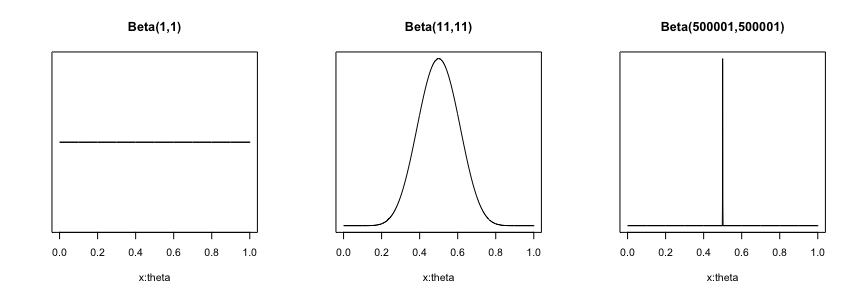
\includegraphics[scale=.3]{beta}
\caption{Beta Distributions}
\label{fig:differentbeta}
\end{figure}

Intuitively, we can think of the first distribution as representing your
state of belief about the probability of getting a head on the next
flip. This distribution is plotted in Figure 1: note that it is wholly
flat, capturing the sort of state of indifference that the Principle of
Indifference is supposed to capture: One finds no ground in thinking one
probability is more credible than another.

The second distribution can be seen as our state of belief after
witnessing 10 flips of the coin, and 5 turn up heads and 5 tails.
Naturally, the peak - the mode of the distribution - is at
\(\theta = 0.5\), which seems sensible, because it reflects the evidence
that exactly half of the samples are heads. But we can see that at this
stage we are quite uncertain about \(\theta\), evidenced by the width of
the distribution. While \(\theta = 0.5\) is the peak, there is a
substantial area covering \(\theta > 0.55\) and \(\theta < 0.45\).

The third distribution, modeling the state of belief after one million
trials with half of them being heads, is intended to be an approximation
of Popper's ideal evidence scenario. The peak is again at \(0.5\), but
this plot has a noticeably narrower spread: we are much more confident
in our assessment that the coin has an equal propensity to land on heads
as tails. Also notice that at this stage, any value of \(\theta\) other
than \(0.5\) are practically impossible after receiving the ideal
evidence.

To state these observations more precisely, we can calculate the exact
probability using the corresponding cumulative distributions. Since beta
distributions are continuous distributions, we can only deal with
intervals of values. Still, we can provide a reasonably close
approximations. For instance, conditional on the ideal evidence, we
would be absolutely sure that the probability is between 0.49 and 0.51. The relevant probabilities are summarized in the
following table:

\begin{longtable}[]{@{}lrr@{}}
\toprule
Distribution & \(P(0.46<\theta<0.54)\) &
\(P(0.49<\theta<0.51)\)\tabularnewline
\midrule
\endhead
\(Beta(1,1)\) & \(0.08\) & \(0.02\)\tabularnewline
\(Beta(11,11)\) & \(0.29\) & \(0.07\)\tabularnewline
\(Beta(500001,500001)\) & \(1\) & \(1\)\tabularnewline
\bottomrule
\end{longtable}

Now, let \(E\) be the ideal evidence, \(X_1,…X_{1000000}\), where
\(\sum_{i=1}^{1000000}X_i = 500000\), and let \(\theta\) be the coin's
propensity to land on heads. We now see that the following inequality
holds, since the left-hand side is \(0.02\), and for the right it's
\(1\).

\[P(0.49<\theta<0.51) <  P(0.49<\theta<0.51|E)\]

To make things more official-sounding, perhaps we can describe this as
\emph{Higher Order Relevance(HOR)}. Recall Keynes's idea is that for
some evidence \(E\) and hypothesis \(H\)

\[\text{Evidence $E$ is relevant to $H$ if and only if }P(H) \neq P(H|E)\]

HOR takes this on step further and suggests that, in addition to \(H\)
and \(E\), consider specific values \(x\) and \(y\), where
\(0 \leq x \leq y \leq 1\)

\[\text{Evidence $E$ has a higher order relevance to $\theta$ iff}\]
\[P(x\leq \theta \leq y) \neq P(x\leq \theta \leq y)|E)\]

Under this analysis, we can see that Popper's argument contains a
sleight of hand that shifts between two ways of thinking about N---the
next coin toss landing on heads---'s probability. The argument begins by
asking, rather innocuously, for your prior for \(N\), but the ideal
evidence \(I\) Popper immediately introduced is not for \(N\) but for
the hypothesis that \(\theta = 0.5\). Popper is reasonably explicit
about \emph{that}, but what he is not explicit about is \emph{this}: he
has convinced us that \(I\) is both evidentially ideal for and
conditionally relevant to \(\theta = 0.5\). That, however, is a
misdirection, because he immediately starts talking the conditional
probability on \(I\), \emph{not} of \(H_{0.5}\), but of \(N\).

While I think that HOR provides a technical response to Popper's
paradox, it is not quite the same as accounting for the phenomenon in
question. In fact, by focusing on overcoming the difficulty raised by
the paradox caused by an absurd amount of evidence, we might have
overlooked what is truly at stake: rarely, if ever, do we have ideal
evidence for any substantive hypothesis, so situations where we have an
overabundance of evidence is an incomplete benchmark for the adequacy of
the account. In fact, our analysis shows that when we have perfect
information, evidential weight essentially becomes a non-issue, because
it eliminates the uncertainty that calls for probabilistic reasoning to
begin with.

The important question, instead, is whether HOR can help with decision
making in situations where evidence is severely lacking. To this end, it
remains to be seen how higher order relevance can trickle down to first
order probability, on which decision making is based within the
classical Bayesian framework.

We need to, then, ask ourselves if HOR as a concept can make any
practical difference in decision making. It is in fact difficult to do
so within the basic framework of Bayesianism. To see this, imagine a
perverse game in which you will be shot to death if a coin flip lands on
head. Clearly, you don't want heads. You are given a choice between two
coins: the first coin \(P\) is similar to Popper's coin from the ideal
evidence scenario, except now the ideal evidence actually shows that
there is a slight bias in favor of heads, say the expected value is
0.51. The other coin \(U\) is one you have never seen before, so on an
ignorance prior your expected value \(E(\theta_U)\) is 0.5 . Now, which
would you choose? An argument can be made that you probably still want
the Popperian coin, because you know you are almost certainly getting
\(\theta_P = 0.51\). From the perspective of expected utility, however,
it is hard to rationalize such a decision, because the unknown coin
still has a lower expected value. That is,

\[\frac{510000}{1000000}> \frac{1}{2}\]

So it seems that we are back to where we started - the relevance
demonstrated on a higher order simply vanishes when we consider the
matter on the level of decision making, which is entirely based on a
precise point-estimate of the first order probability.

If the point estimate is to be blamed, the natural response is that we
do rely on an interval estimate instead. This solution is reminiscent of
the call to abolish the use of \(p\) values in Frequentist statistics,
and instead we should report the confidence interval of our findings.
The idea is that point estimates are inherently misleading, since they,
by design, summarize the data by discarding information such as higher
order relevance. This problem is somewhat analogous to the one we are
running into with respect to expected values. So one possible solution
is that we should only insist on making our decisions based on
\emph{credible intervals}, which is the Bayesian version of the
confidence interval. For instance, suppose
\(\theta_P \sim Beta(480000,520000)\) and \(\theta_U \sim Beta(1,1)\).
We can deduce that

\[P(0.479\leq \theta_P \leq 0.481) = 0.99\]
\[P(0.005\leq \theta_U \leq 0.995) = 0.99\]

\noindent In other words, we can say there is a 0.99 probability that
\(P\)'s propensity to land on heads is between 0.479 and 0.481
(practically 0.48) and for \(U\) it's between 0.005 and 0.995.

However, it seems to me that we are simply restating higher order
relevance in terms of credible intervals, without dealing with the crux
of the problem - unless we are rationally allowed to refuse to follow
the precise expected value, even if the weight of evidence is low, we
will always have to match it to our best point estimate, which is the
expected value. Of course, the point is not that HOR doesn't matter,
because intuitively it does. The point is rather that we need a richer
philosophical framework to rationalize this intuition.

\hypertarget{the-concept-of-resiliency-1}{%
\section{The Concept of
Resiliency}\label{the-concept-of-resiliency-1}}

Skyrms credits Richard Jeffrey as the first who notices that Popper's
paradox brings light to the very idea of resiliency.\footnote{\cite{causationandconditional},704} Jeffrey points out
that once we stop fixating on the probability of \(N\), the next toss
coming up head, we can see that our state of belief prior receiving the
ideal evidence has a degree of malleability.\footnote{\cite{jeffreydecision}, 184.} Consider, for instance, instead of
asking only for the probability of \(N\), we ask the probability of the
next 5 tosses coming up heads. Once we think about how our belief
responds to how these 5 tosses would act as potential evidence, given
our posterior state of belief, we have very little choice but to believe
that probability is \((0.5)^5\), but we would be a lot less compelled to
do so with the prior state of belief.

Skyrms has proposed the notion of \emph{resiliency} to capture Jeffrey's
observation in a generalized manner: even though evidential weight is
not reflected by the probability, it is captured by its stability.\footnote{\cite{causationandconditional}, 705} The
idea that there is a probabilistic representation for a stable state of
belief can be illustrated as follows: if I have in front of me an urn
\(U\), with an unknown proportion of black and white balls. If I
randomly draw 2 balls from it with replacement and find one ball for
each color, my intuitive estimate of the proportion of black balls would
sensibly be somewhere around 1/2. But my state of belief should be
relatively unstable: it would be irrational for me to fixate on this
estimate, especially new light of conflicting evidence. If I sample two
more balls from the urn and they are both black, it would make sense for
me to raise my estimate for the proportion of black balls to more than
1/2---perhaps to 3/4. But suppose I continue to sample from for 996 more
times. Out of the total 1000 draws, 500 are black. At this point a
sensible would be back to around 1/2, but unlike my state of belief
after only 2 samples, after 1000 samples my state of belief is
stabilized: suppose I sample again and I draw five black balls in a row.
Now, even though drawing 5 black balls in a row seems rather
extraordinary, against the body of my evidence it would not warrant me
to revise my belief in any significant measure.

The intuition here is that the increase in the amount of evidence,
expressed here in terms of the number of samples, corresponds to the
increase of stability of the estimate. Skyrms has introduced a notion
called the \emph{resiliency} to capture this intuition sense of
stability.

Conceptually, this is an attractive way to capture to notion of
evidential weight. Keynes' puzzlement about how relevance and weight
could come apart is addressed; When a belief \(B\) is resilient, the
conditional probability on some new evidence \(E\) should be
approximately the same, that is, \(P(B|E) \approx P(B)\), even if \(E\)
would be highly relevant were \(B\) not resilient. If, for instance, a
resilient belief is one where the weight of the evidence for it is high,
then it is a logical consequence that evidence could make a belief more
weighty without changing its degree, for the weight is in fact
stabilizing this particular value.

Nevertheless, how the resilience of a belief can make a practical
difference is yet to be explained. In fact, for the most part,
resiliency does not do much better than higher order relevance: within
the structure of expected utility calculus, a highly resilient belief
will still recommend the same action as a non-resilient belief with the
same expected value. Skyrms' original motivation for the concept,
however, provides an important clue: he intended the concept of
resiliency to explicate the concept of the laws of nature, so the idea
is that a probability statement \(A\) based on a law of nature is one
that remains resilient against various extreme scenarios. What this
means is that we are supposed to calculate likelihoods based on data
that \emph{might have happened}, and see whether \(A\) is resilient
against it.\footnote{James Joyce has recently proposed that what evidential weight does is to stabilize the distance between one's subjective probability of an event and her underlying hypotheses of the objective chance about it. Joyce's account has some important technical advantage, but conceptually it remains the same as Skyrms' account. Essentially, Joyce's suggestion is that the basic resilient quantity is the \emph{expected loss} of a particular chance hypothesis. Providing a proper treatment would require an exposition on statistical decision theory, so I have decided to omit it here. See \cite{joycehpre}, 166-168.}



\hypertarget{counterfactual-priors-and-hypothetical-data-1}{%
\section{Counterfactual Priors and Hypothetical
Data}\label{counterfactual-priors-and-hypothetical-data-1}}

The notion of resiliency opens the door to how counterfactual reasoning
can be relevant in Bayesian reasoning. The crucial point is that to see
how resilient a probability is, it is not something we can determine by
looking at data that we already have. We have examine what \emph{might
have happened}. So notwithstanding Lindley's rhetorical question:

\begin{quote}
Of what relevance are things that might have happened, but did
not?\footnote{\cite{lindleybern}, 114.}
\end{quote}

Counterfactual considerations are relevant in deliberating on how a
chosen hypothesis \emph{would} respond in light of confounding
scenarios, so that we can decide if it is a worthy hypothesis and, if
chosen, how we ought to further probe it. More specifically, the weight
of evidence is puzzling, because it needs to be understood in the
context of abduction, since its goal is to give information about how we
ought to structure our inductive space.

Skyrms suggests that the resilience of a belief manifests itself as ``a
reluctance to change.''\footnote{\cite{causationandconditional}, 707.} He suggests that we can measure weight
directly in terms of the difference between prior and posterior
probabilities. Perhaps we can call this the measure of instability,
which signifies a lack of weight:

\[\text{Instability: }|P(X|E_j) - y|\]

Where \(j\) is in the set of \(n\) possible states of affairs,
\(E_1,..., E_n\). Skyrms' idea is that we should pick a \(j\) that
creates the biggest difference.

To see what this means, consider how resiliency can be demonstrated
using the beta distribution, though keep in mind that it is not meant to
be a generalizable result, since different distributions work
differently. In any case, recall that different sets of parameters can
produce the same expected value. For instance, consider \(Beta(1,1)\)
and \(Beta(5000,5000)\). Their expected values are, of course, the same,
since \(\frac{1}{2} = \frac{5000}{10000}\). But the second distribution
is way much resilient than the first. Suppose these are distribution
functions that represent the opinions of two different agents, but they
both receive the same piece of evidence \(Y\) from a Bernoulli process
such that \(Y=\sum_{i=1}^5 X_i=5\), that is, getting 5 heads in a row.
We do not have to do the calculation to see that they will respond to
the evidence pretty differently: the first agent will raise her
posterior expected value from \(1/2\) to \(6/7\). The difference is
\(.36\), which is a considerable increase.

The second agent's opinion, however, would barely be changed:

\[\frac{5005}{10005} - \frac{5000}{10000} = 0.00025\]

It is barely a rounding error. In fact, we can see that the second agent
would have to see 200 successes \emph{in a row} in order to raise the
credence by \(0.01\):

\[\frac{5000+200}{5000+5000+200} = 0.51\]

Notice that this analysis requires counterfactual thinking in two ways:
we have to consider what our priors \emph{would} be like in different
circumstances, and we have to consider its response to some hypothetical
data. This is why the weight of evidence is a dispositional commitment:
one is committed to respond to the the deliverance of experience in a
deliberate manner, as dictated by the model decided upon after
considering various counterfactual scenarios.

This way of understanding evidential weight provides an important
insight on the voluntaristic idea that degrees of belief ought to be
understood as taking up an epistemic commitment during the context of
abduction. To deliberate on the appropriate hypothesis to be accepted
provisionally, I have to know what \emph{practical difference} its
acceptance would make on my future conduct. To do so, I have to draw
deductive inferences based on various possible models that I could
possibly accept, based on various hypothetical scenarios that come up
during experiment.

To see what I mean, it might help to see the interaction between the
evidence and posterior probability directly---this is shown in the
figure. The x-axis represents the number of heads in a row, so the
higher x is, the more extreme the hypothetical evidence is. The y-axis
is the posterior probability after receiving the x heads out of x throws
as indicated by the x-axis.

\begin{figure}
\centering
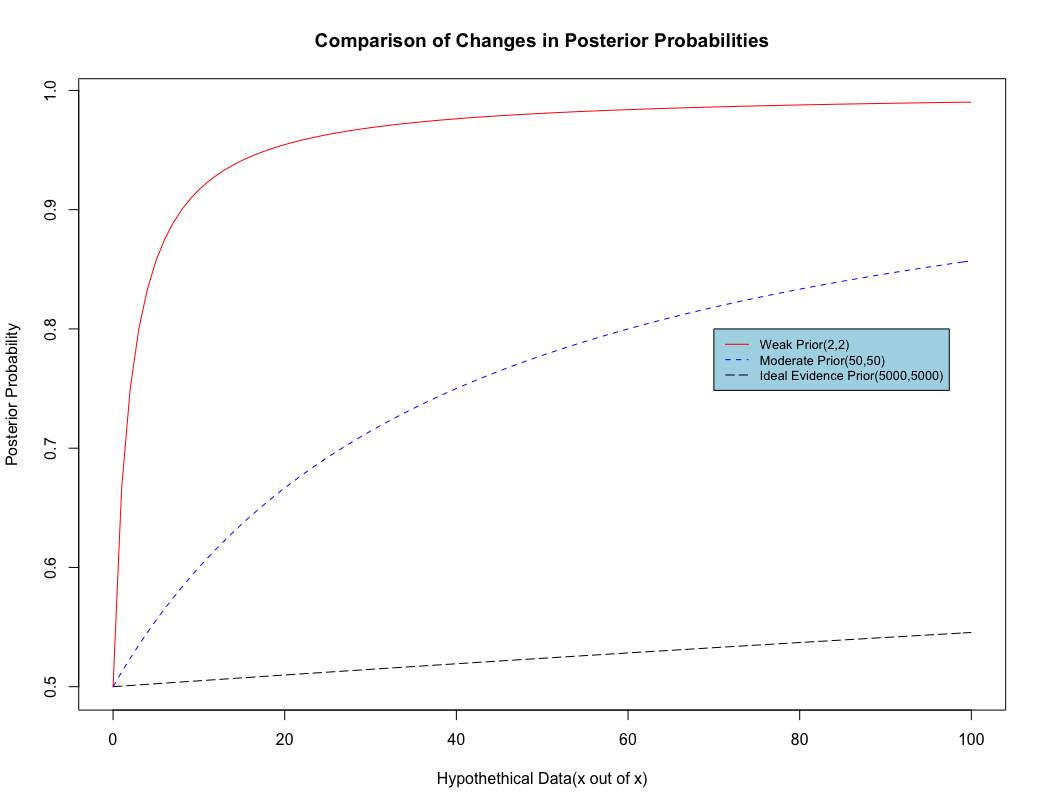
\includegraphics[scale=0.3]{rescompare}
\caption{Comparison of stabilities of different prior distributions:
values in parentheses are parameters for the beta distribution.}
\label{fig:res}
\end{figure}

We see that these counterfactual priors behave quite differently in
slight of extreme evidence. Here, the weight of evidence clearly
corresponds to the sum of the parameters \(\alpha + \beta\), and the
higher it is, the less responsive it is to evidence. This is especially
clear when \(\alpha = \beta = 500\)---we see that with such as a weighty
prior distribution, it makes absolutely no difference how the extreme
the data is, until we get more than 60 heads in a row. Even if we tossed
100 out of 100, the expected value stays very close to \(0.5\). A ``flat
prior'', i.e., \(\alpha = \beta = 1\), is, as expected, not resilient
against almost any form of extreme evidence. The posterior is expected
to almost \(0.8\) after seeing 10 heads in a row, and rapidly approaches
unity.

From the deliberativist point of view, there is no \emph{a priori}
justification for one over another. There are circumstances in which the
extremely recalcitrant prior would be appropriate. Perhaps we can
consider the probability of a person's guilt based on the evidence. In
such a case, it would be rational to adopt a prior that is extremely
resilient, so that the posterior would be unresponsive unless the
evidence is beyond any reasonable doubt. Even in a less dramatic
situation such as testing the effectiveness of a drug, a resilient prior
could still be advisable when the result could mean have life-altering
consequences.

This also has an implication on the voluntarist interpretation of
degrees of belief. Recall that van Fraassen argues that assertions of
probability should not be a description of the agent's psychological
state. An argument for the voluntarist reading can be made in this
context. Suppose personally I think the coin is extremely likely to be
fair. It seems \emph{less} rational for me to adopt a prior to reflect
such a state, e.g., \(Beta(500,500)\); because, it would look as though
I am rigging the experiment in favor of \emph{my} hypothesis. The
rational thing, as a matter of fact, should be the opposite:
\emph{because} I am confident that my opinion is true, I am
intentionally adopting the opposite prior, with the assumption that the
data will overwhelm it. This is akin to a gambler with inside
information who is willing to make a bet with extremely unfavorable
odds. As the psychologist John Kruschke points out, it might be
advisable to choose a prior to satisfy a skeptic.\footnote{\cite{bayessupert}, 575.}
%
%More important, the deliberativist point of view dovetails Gelman and Shalizi's idea that prior and posterior distributions are \emph{testable}.\footnote{\cite{gelman}, 19} Their idea is that the models, i.e., the distributions, can be examined by comparing hypothetical data generated from them against what is actually observed. Their idea is that if the posterior model is well-fitted, we ought to see 

 
\section{Conclusion}\label{woeconclusion}

The central concern of this chapter is the dynamic between the abductive and deductive contexts of inquiry. We saw that Peice makes the tantalizing suggestion that abduction is \emph{interrogative}. To explain what this means, I borrowed Hintikka's helpful connection between the economics of choosing a hypothesis for inductive testing and choosing an assumption for premiseless proofs. Both involve a strategic element in thinking about the deductive implication of what \emph{would} happen, had the choice been made a certain way. I tried to apply this insight on Keynes' idea of the weight of evidence, and suggested that the evidential weight represents a \emph{dispositional commitment}, revealed through a deductive probability calculus from the chosen prior. We saw that in the case of Popper's paradox of ideal evidence, what has been changed is not the posterior probability, but our willing ness to revision in light of new evidence.  


